\section{Efficient Word Learning Experiments}
We first set out to model the infant learning tasks described in \cite{Smith2002} using
simple neural network models. In order to do so, we use artificial toy data that is designed
to mimic the training data described in the paper. Each object sample is assigned a shape,
texture and color value. There are two types of model evaluations performed, both drawn from
\cite{Smith2002}.

{\bf1. First-order generalization test}: For the first-order generalization test, infants
are asked to evaluate novel instances of familiar objects. To simulate this test, we train
our neural network models to classify objects, ensuring that objects of the same category
are assigned the same shape. Then, we build a test set by creating one novel exemplar of
each category that appeared in the training set. The novel exemplar has the same
shape as the training exemplars of that category, but a new color and texture combination.
Accuracy is defined as the fraction of test images that are correctly classified by the model.
This test is repeated for different training set sizes, i.e. different combinations of
\{\textit{\# categories}, \textit{\# exemplars}\}. It is important to note that as
\textit{\# categories} increases, the first-order task becomes more difficult.

{\bf2. Second-order generalization test}: For the second-order generalization test, infants
are presented with an exemplar of a novel object category as a baseline. Then, they are
shown 3 comparison objects: one which has the same shape as the baseline, one with the same
color, and one with the same texture. In each case, the other 2 features are different from
the baseline. The infants are asked to select which of the 3 comparison objects are of the
same category as the baseline object. We simulate this test by creating an evaluation set
containing groupings of 4 samples: the baseline, the shape constant, the color constant, and
the texture constant. Each grouping serves as one test example. We find which of the 3
samples the NN thinks to be most similar by evaluating the cosine similarity using the
hidden layer features of the model. Accuracy is defined as the fraction of groupings for
which the model chose the correct (shape-similar) object. This test was repeated for
different training set sizes, i.e. different combinations of \{\textit{\# categories},
\textit{\# exemplars}\}.

\begin{figure*}[h]
    \begin{center}
        % mlp results
        \begin{subfigure}[b]{0.47\textwidth}
            \begin{center}
                % subfigure (a)
                \begin{subfigure}[b]{0.48\textwidth}
                    \begin{center}
                        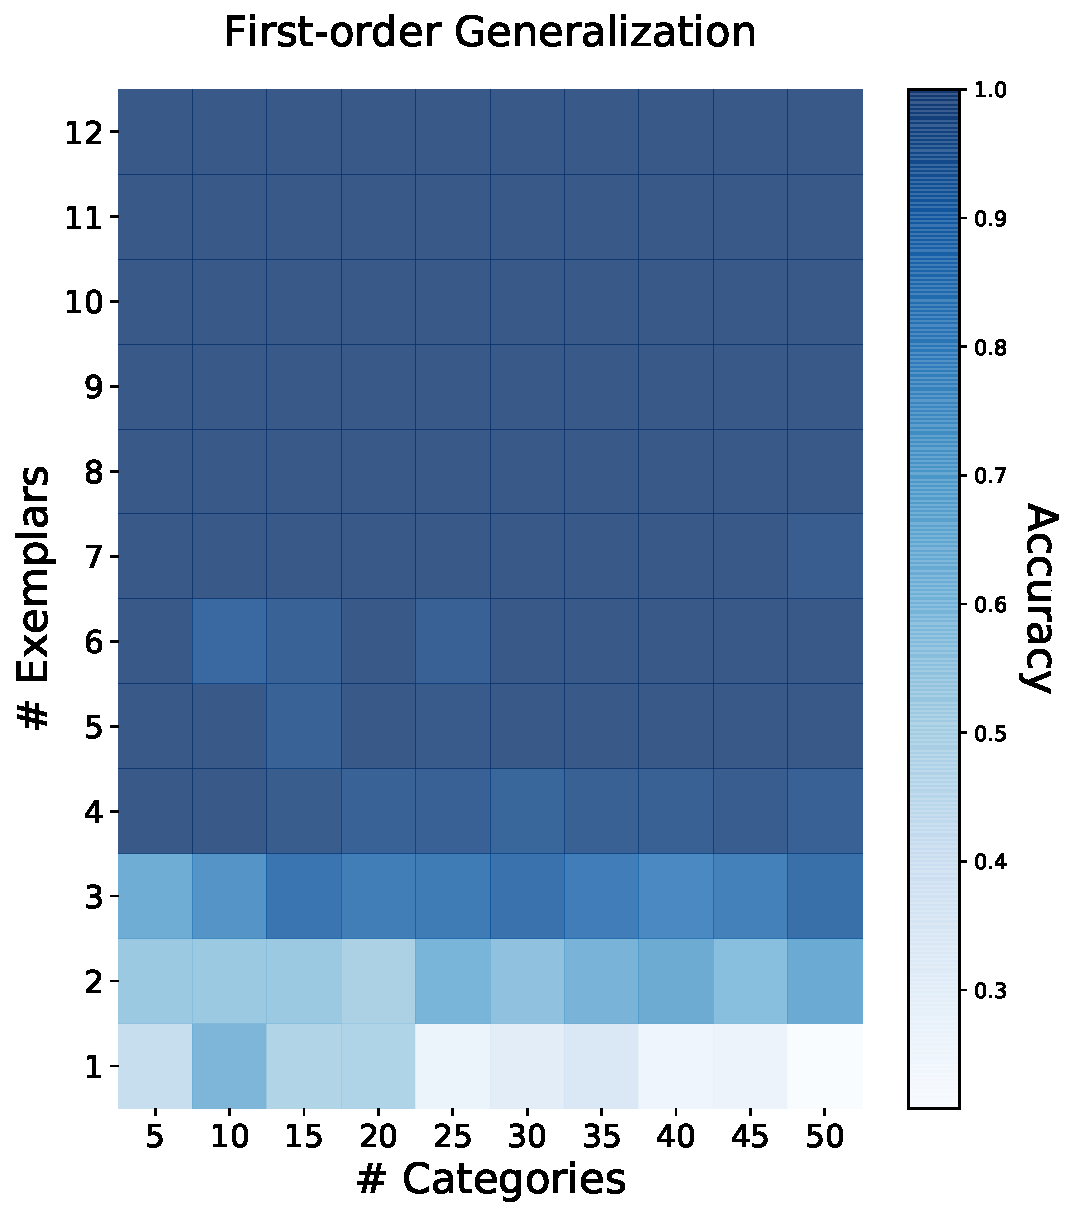
\includegraphics[width=0.98\textwidth]{figures/mlp_1order_accuracy.pdf}
                    \end{center}
                \end{subfigure}
                % subfigure (b)
                \begin{subfigure}[b]{0.48\textwidth}
                    \begin{center}
                        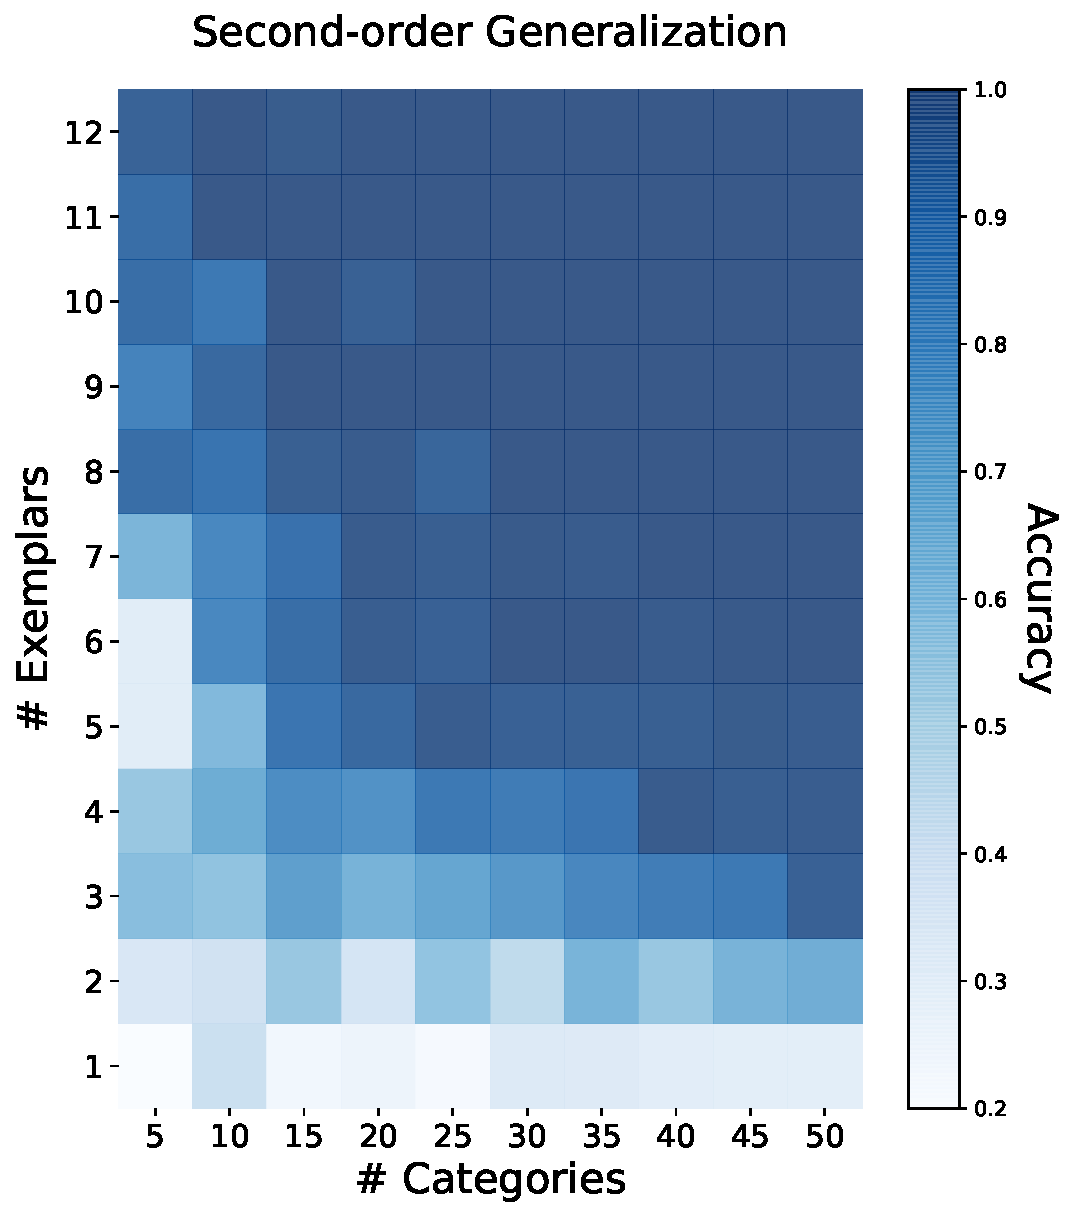
\includegraphics[width=0.98\textwidth]{figures/mlp_2order_accuracy.pdf}
                    \end{center}
                \end{subfigure}
            \end{center}
            \caption{MLP}
            \label{mlp_results}
        \end{subfigure}
        % cnn results
        \begin{subfigure}[b]{0.47\textwidth}
            \begin{center}
                % subfigure (a)
                \begin{subfigure}[b]{0.48\textwidth}
                    \begin{center}
                        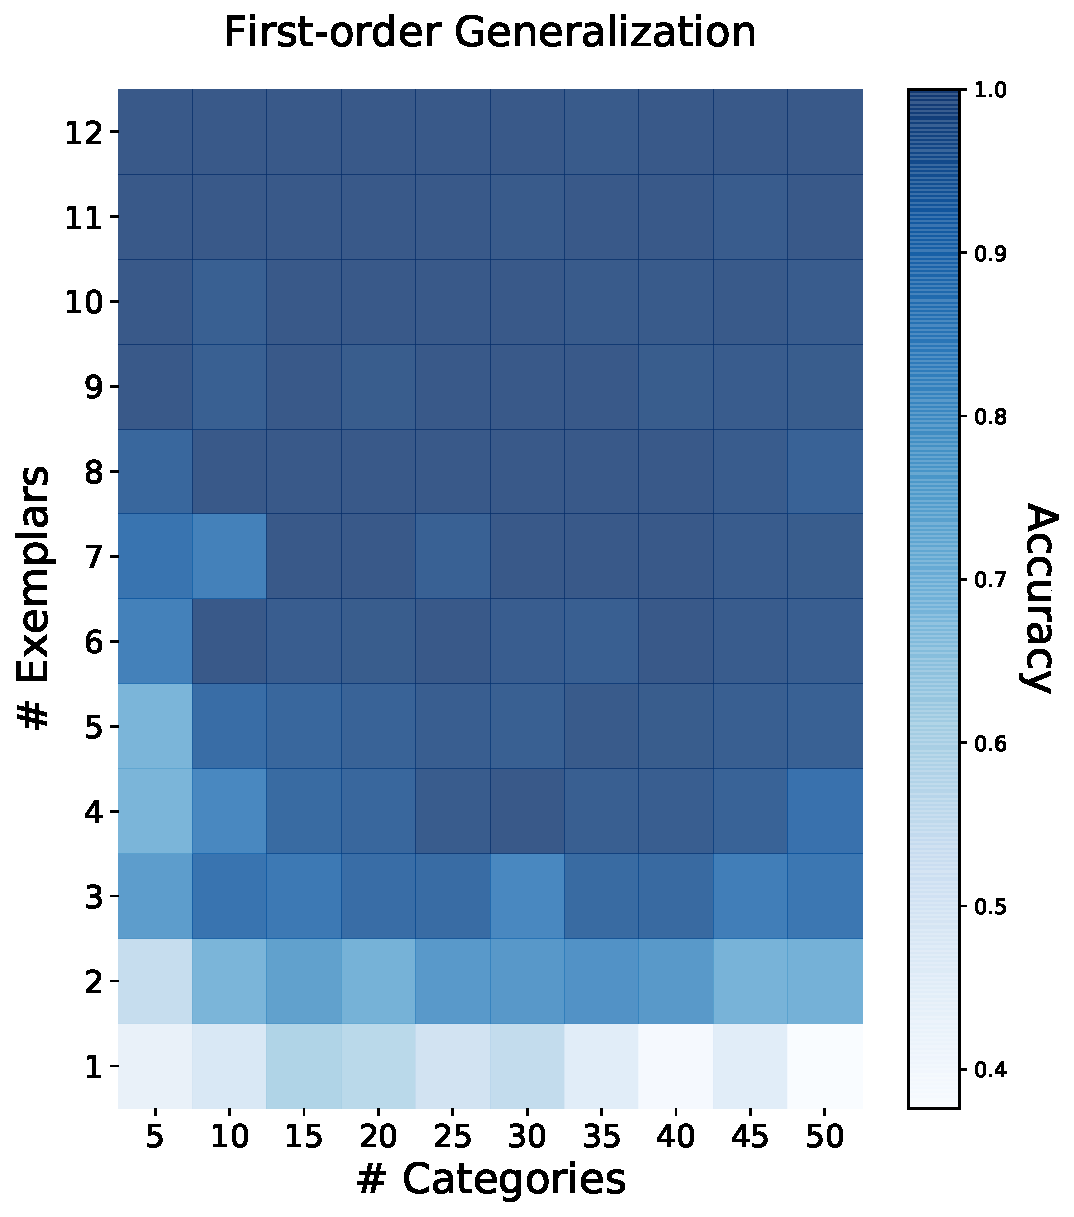
\includegraphics[width=\textwidth]{figures/cnn_1order_accuracy.pdf}
                    \end{center}
                \end{subfigure}
                % subfigure (b)
                \begin{subfigure}[b]{0.48\textwidth}
                    \begin{center}
                        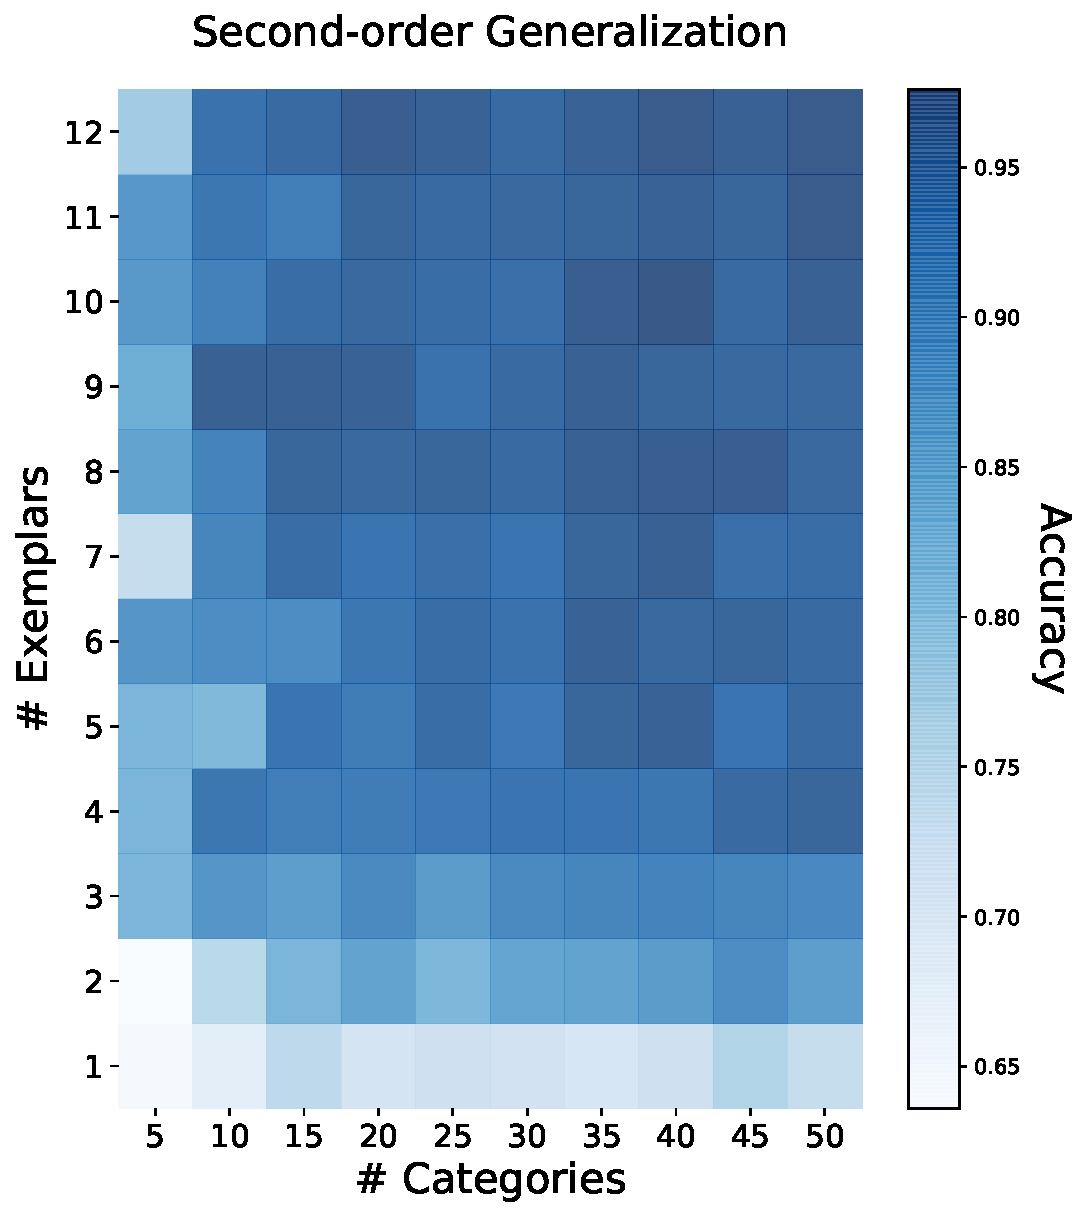
\includegraphics[width=\textwidth]{figures/cnn_2order_accuracy.pdf}
                    \end{center}
                \end{subfigure}
            \end{center}
            \caption{CNN}
            \label{cnn_results}
        \end{subfigure}
    \end{center}
    \caption{First- and second-order generalization results for the simple MLP and CNN models.
    For each \{\textit{\# categories}, \textit{\# exemplars}\} pair, the average result from
    5 trials is shown.}
    \label{generalization_results}
\end{figure*}

% \begin{figure}[h!]
%     % subfigure (a)
%     \begin{subfigure}[b]{0.25\textwidth}
%         \begin{center}
%             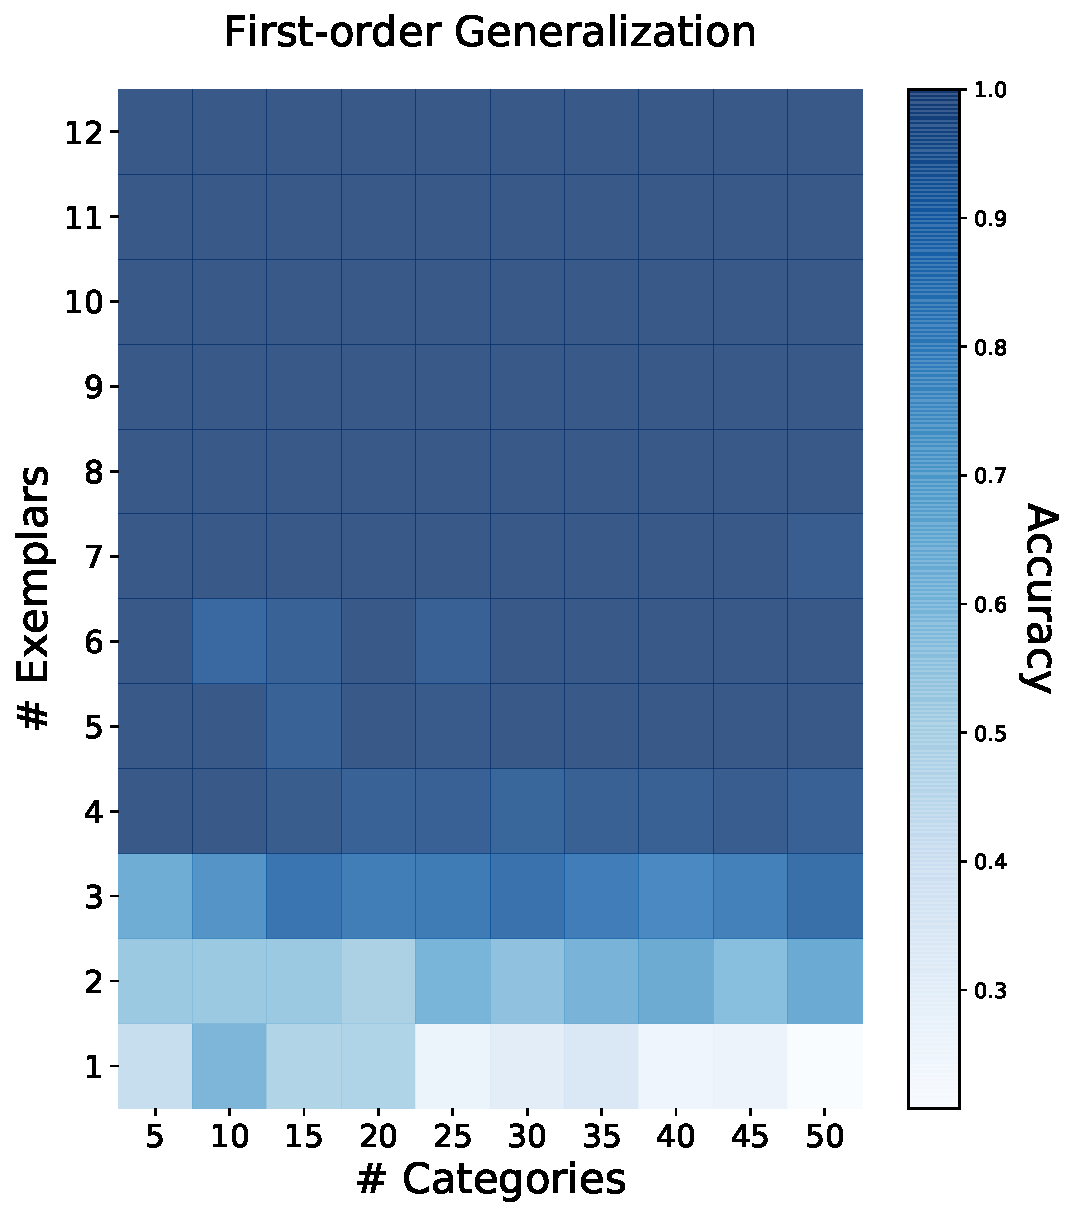
\includegraphics[width=0.98\textwidth]{figures/mlp_1order_accuracy.pdf}
%         \end{center}
%         \label{fig:mlp_1order_results}
%     \end{subfigure}
%     % subfigure (b)
%     \begin{subfigure}[b]{0.25\textwidth}
%         \begin{center}
%             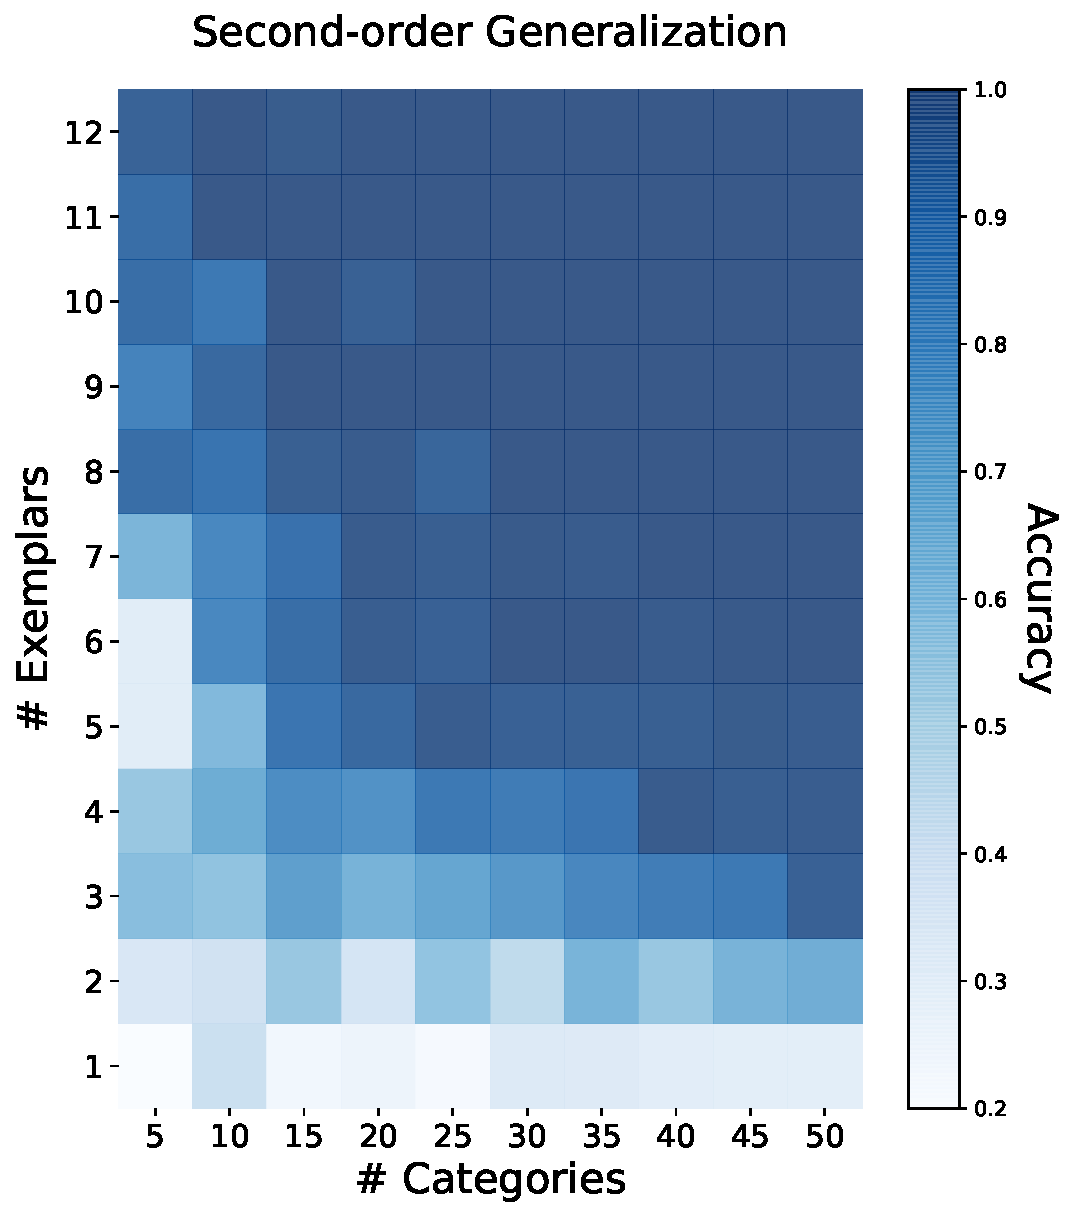
\includegraphics[width=0.98\textwidth]{figures/mlp_2order_accuracy.pdf}
%         \end{center}
%         \label{fig:mlp_2order_results}
%     \end{subfigure}
%     % caption
%     \caption{MLP first- and second-order generalization results. For each
%     \{\textit{\# categories}, \textit{\# exemplars}\} pair, the average result from 5 trials
%     is shown.}
%     \label{fig:mlp_results}
% \end{figure}

% \begin{figure}[h!]
%     % subfigure (a)
%     \begin{subfigure}[b]{0.25\textwidth}
%         \begin{center}
%             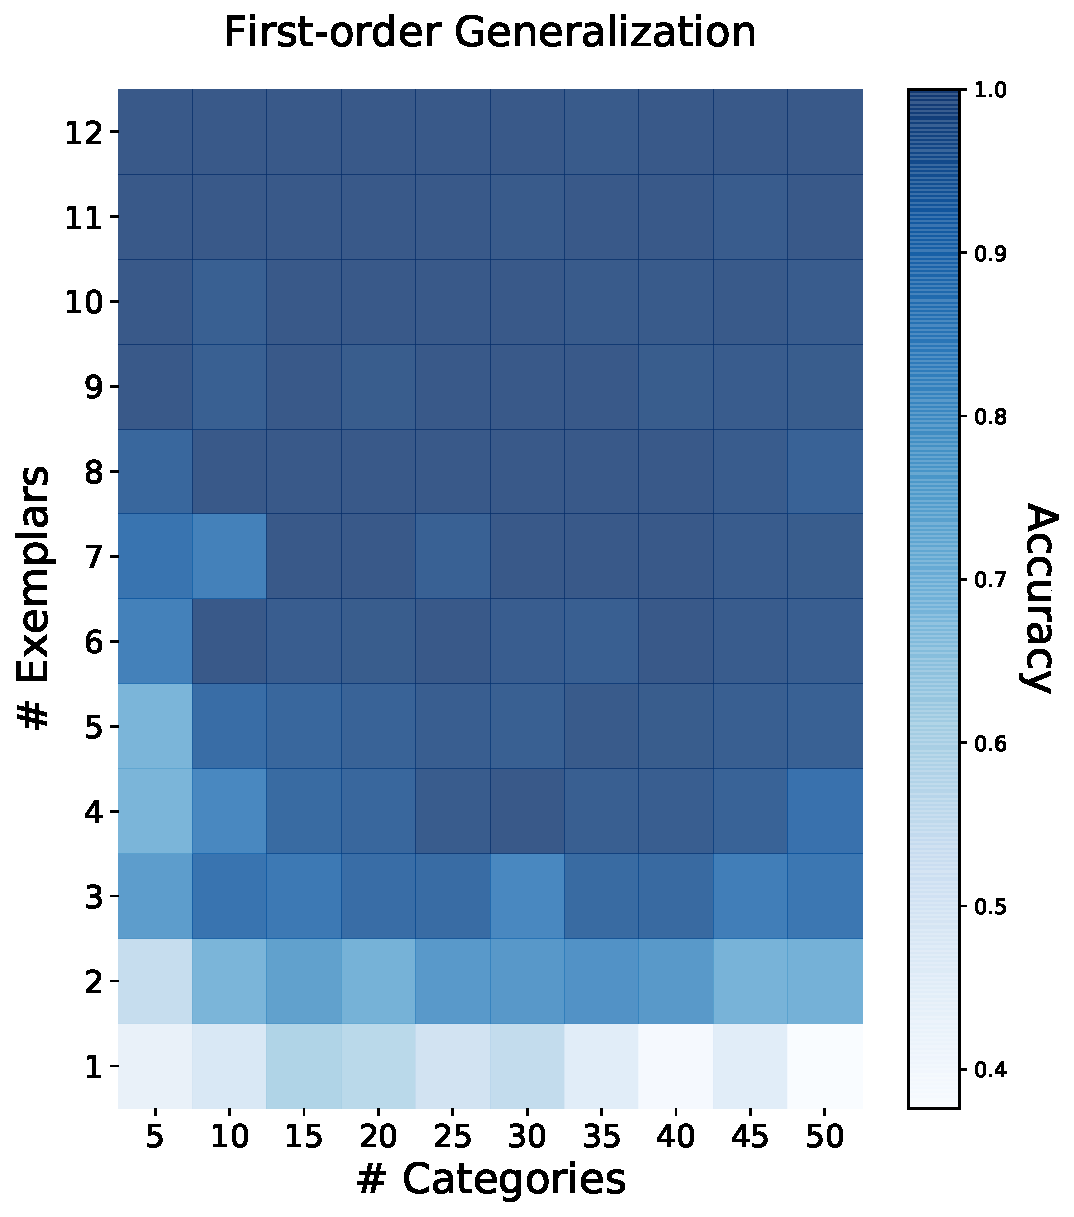
\includegraphics[width=0.98\textwidth]{figures/cnn_1order_accuracy.pdf}
%         \end{center}
%         \label{fig:mlp_1order_results}
%     \end{subfigure}
%     % subfigure (b)
%     \begin{subfigure}[b]{0.25\textwidth}
%         \begin{center}
%             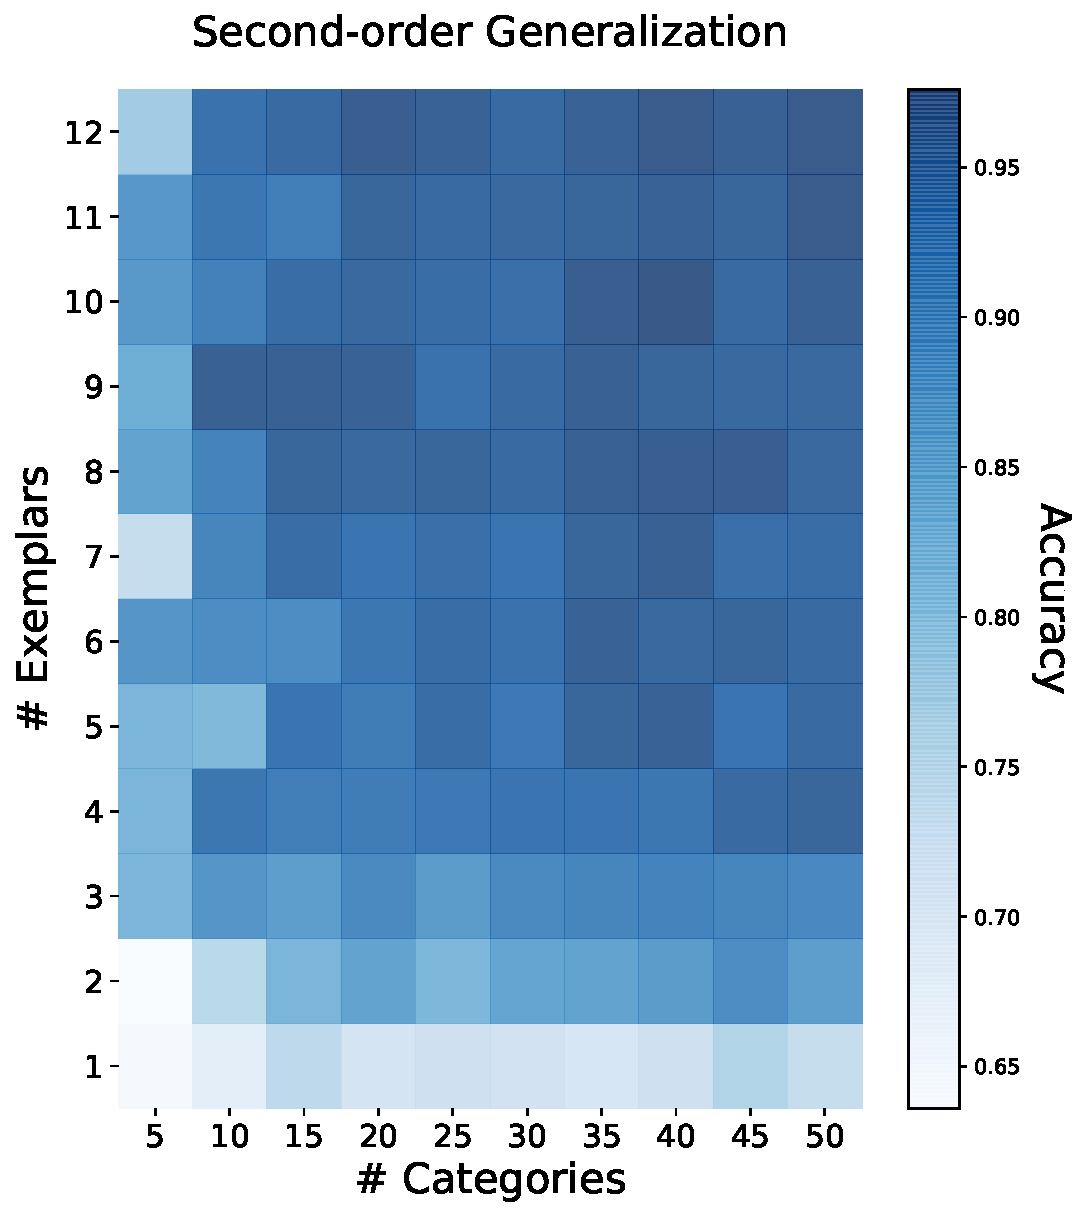
\includegraphics[width=0.98\textwidth]{figures/cnn_2order_accuracy.pdf}
%         \end{center}
%         \label{fig:mlp_2order_results}
%     \end{subfigure}
%     % caption
%     \caption{CNN first- and second-order generalization results. For each
%     \{\textit{\# categories}, \textit{\# exemplars}\} pair, the average result from 5 trials
%     is shown.}
%     \label{fig:mlp_results}
% \end{figure}

\subsection{Simple Multilayer Perceptron}
To begin with, we use a simple multilayer perceptron (MLP) that operates on categorical
data. Since shape, color, \& texture have categorical feature values, we encode the values
using unique bit vectors that are randomly assigned at the beginning of the experiment. We
use a simple feed-forward NN with one hidden layer of 30 units, and the ReLU activation
function. The number of units in the softmax layer depends on the \textit{\# categories}
parameter for the particular dataset. Results are shown in Fig. \ref{mlp_results}.

\subsection{Simple Convolutional Neural Network}
As a second type of model, we used a simple convolutional neural network (CNN) architecture
consisting of... TODO. To train this CNN, we generated images of artificial 2-D objects
(Fig. \ref{generated_images}) with a variety of different shape, color and texture values. TODO... finish.
Results are shown in Fig. \ref{cnn_results}.

\begin{figure}[h!]
    % shape 1
    \begin{subfigure}[b]{0.4\textwidth}
        \begin{center}
            \begin{subfigure}[b]{0.48\textwidth}
                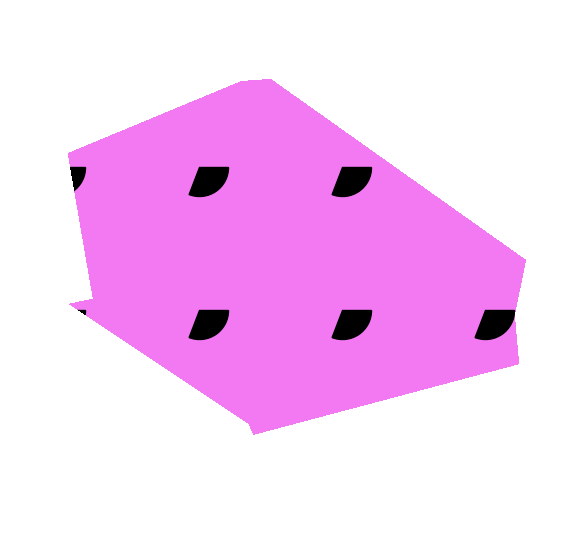
\includegraphics[width=\linewidth]{figures/img0000.png}
            \end{subfigure}
            \begin{subfigure}[b]{0.5\textwidth}
                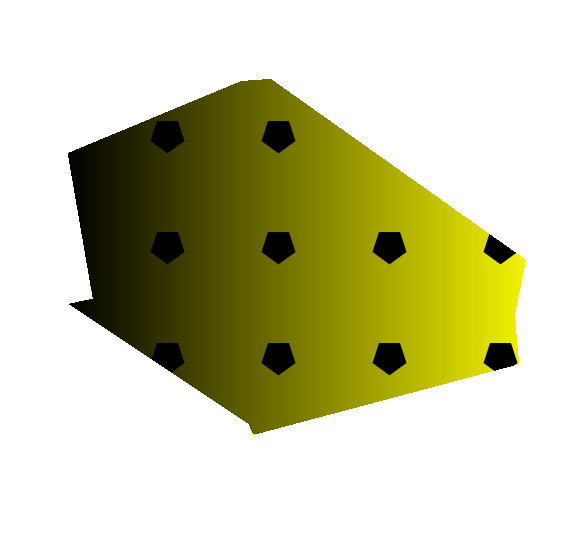
\includegraphics[width=\linewidth]{figures/img0001.png}
            \end{subfigure}
        \end{center}
    \end{subfigure}
    % % shape 2
    \begin{subfigure}[b]{0.4\textwidth}
        \begin{center}
            \begin{subfigure}[b]{0.48\textwidth}
                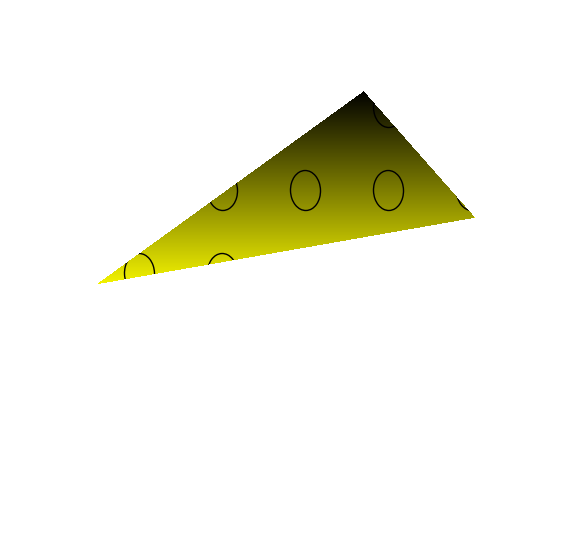
\includegraphics[width=\linewidth]{figures/img0002.png}
            \end{subfigure}
            \begin{subfigure}[b]{0.5\textwidth}
                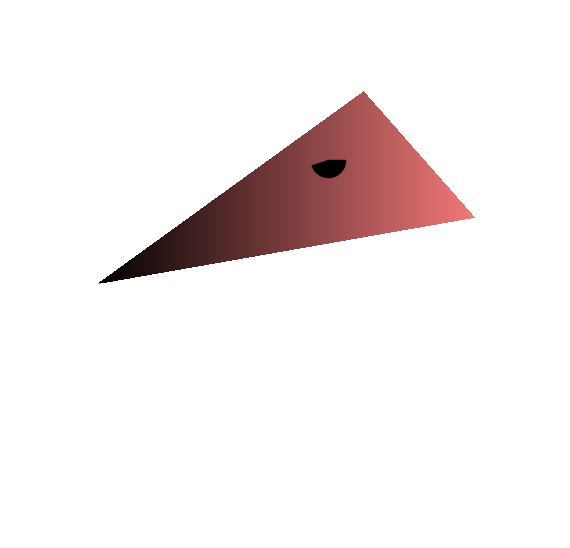
\includegraphics[width=\linewidth]{figures/img0003.png}
            \end{subfigure}
        \end{center}
    \end{subfigure}
    \begin{subfigure}[b]{0.4\textwidth}
        \begin{center}
            \begin{subfigure}[b]{0.48\textwidth}
                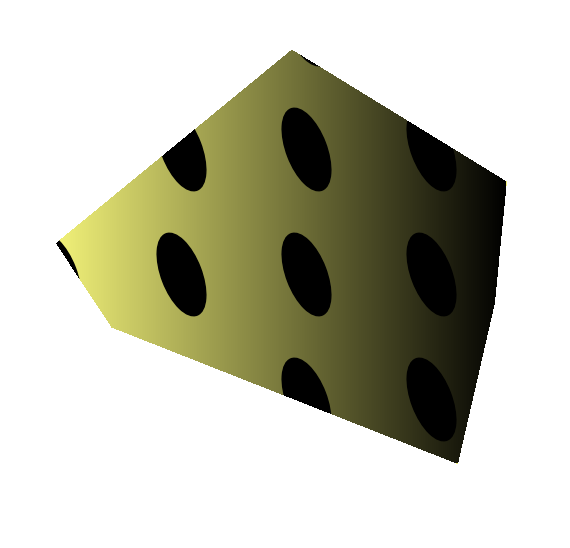
\includegraphics[width=\linewidth]{figures/img0004.png}
            \end{subfigure}
            \begin{subfigure}[b]{0.5\textwidth}
                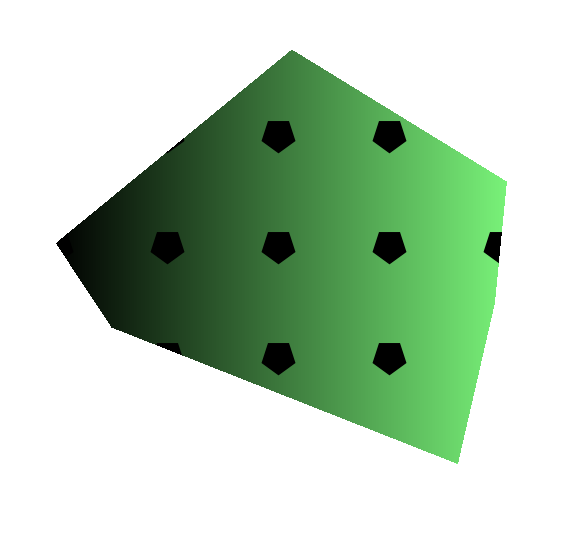
\includegraphics[width=\linewidth]{figures/img0005.png}
            \end{subfigure}
        \end{center}
    \end{subfigure}
    \caption{Images of artificial 2D objects with different shape, color and texture features.}
    \label{generated_images}
\end{figure}



\newpage
\section{Layer-wise Bias Analysis}

